\documentclass{beamer}
\mode<presentation>
\usepackage{amsmath}
\usepackage{amssymb}
\usepackage{algorithmic}
%\usepackage{advdate}
\usepackage{adjustbox}
\usepackage{subcaption}
\usepackage{enumitem}
\usepackage{multicol}
\usepackage{mathtools}
\usepackage{listings}
\usepackage{url}
\def\UrlBreaks{\do\/\do-}
\usetheme{Boadilla}
\usecolortheme{lily}
\setbeamertemplate{footline}
{
	\leavevmode%
	\hbox{%
		\begin{beamercolorbox}[wd=\paperwidth,ht=2.25ex,dp=1ex,right]{author in head/foot}%
			\insertframenumber{} / \inserttotalframenumber\hspace*{2ex} 
	\end{beamercolorbox}}%
	\vskip0pt%
}
\setbeamertemplate{navigation symbols}{}

\providecommand{\nCr}[2]{\,^{#1}C_{#2}} % nCr
\providecommand{\nPr}[2]{\,^{#1}P_{#2}} % nPr
\providecommand{\mbf}{\mathbf}
\providecommand{\pr}[1]{\ensuremath{\Pr\left(#1\right)}}
\providecommand{\qfunc}[1]{\ensuremath{Q\left(#1\right)}}
\providecommand{\sbrak}[1]{\ensuremath{{}\left[#1\right]}}
\providecommand{\lsbrak}[1]{\ensuremath{{}\left[#1\right.}}
\providecommand{\rsbrak}[1]{\ensuremath{{}\left.#1\right]}}
\providecommand{\brak}[1]{\ensuremath{\left(#1\right)}}
\providecommand{\lbrak}[1]{\ensuremath{\left(#1\right.}}
\providecommand{\rbrak}[1]{\ensuremath{\left.#1\right)}}
\providecommand{\cbrak}[1]{\ensuremath{\left\{#1\right\}}}
\providecommand{\lcbrak}[1]{\ensuremath{\left\{#1\right.}}
\providecommand{\rcbrak}[1]{\ensuremath{\left.#1\right\}}}
\theoremstyle{remark}
\newtheorem{rem}{Remark}
\newcommand{\sgn}{\mathop{\mathrm{sgn}}}
\providecommand{\abs}[1]{\left\vert#1\right\vert}
\providecommand{\res}[1]{\Res\displaylimits_{#1}} 
\providecommand{\norm}[1]{\lVert#1\rVert}
\providecommand{\mtx}[1]{\mathbf{#1}}
\providecommand{\mean}[1]{E\left[ #1 \right]}
\providecommand{\fourier}{\overset{\mathcal{F}}{ \rightleftharpoons}}
%\providecommand{\hilbert}{\overset{\mathcal{H}}{ \rightleftharpoons}}
\providecommand{\system}{\overset{\mathcal{H}}{ \longleftrightarrow}}
%\newcommand{\solution}[2]{\textbf{Solution:}{#1}}
%\newcommand{\solution}{\noindent \textbf{Solution: }}
\providecommand{\dec}[2]{\ensuremath{\overset{#1}{\underset{#2}{\gtrless}}}}
\newcommand{\myvec}[1]{\ensuremath{\begin{pmatrix}#1\end{pmatrix}}}
\let\vec\mathbf

\lstset{
	%language=C,
	frame=single, 
	% breaklines=true,
	columns=fullflexible
}

\numberwithin{equation}{section}

\title{Solve the differential equation and Verify the solution}
\author{Eshan Sharma - EE24BTECH11022}

\date{\today} 
\begin{document}
	
	\begin{frame}
		\titlepage
	\end{frame}
	
	\section*{Outline}
	\begin{frame}
		\tableofcontents
	\end{frame}
	
	\section{Problem}
	\begin{frame}
		\frametitle{Problem Statement}
		Solve the differential equation,
		\begin{align}
			\frac{d^2y}{dx^2} + y = 0
		\end{align}
		with inital conditions $x=0$ and $y=0$
	\end{frame}
	
	%\subsection{Literature}
	\section{Solution}
	
	\subsection{Laplace Transform Solution}
	\begin{frame}[allowframebreaks]
		\frametitle{Laplace Transform Solution}
		Given:
		\begin{align}
			\frac{d^2y}{dx^2} + y &= 0
		\end{align}
		Taking the Laplace Transform of both sides:
		\begin{align}
			\mathcal{L}\left\{\frac{d^2y}{dx^2}\right\} + \mathcal{L}\{y\} &= \mathcal{L}\{0\}
		\end{align}
		Using properties of the Laplace Transform:
		\begin{align}
			s^2Y(s) - sy(0) - y'(0) + Y(s) &= 0
		\end{align}
		Substituting the initial conditions \( y(0) = C_1 \) and \( y'(0) = C_2 \):
		\begin{align}
			s^2Y(s) - sC_1 - C_2 + Y(s) &= 0\\
			\left(s^2 + 1\right)Y(s) &= sC_1 + C_2\\
			Y(s) &= \frac{sC_1 + C_2}{s^2 + 1}
		\end{align}
		
		The Region of Convergence (ROC) is the entire \( s \)-plane since \( s^2 + 1 \neq 0 \) for all real \( s \).\\
		Taking the inverse Laplace Transform:
		\begin{align}
			y(x) &= \mathcal{L}^{-1}\left\{\frac{sC_1 + C_2}{s^2 + 1}\right\}\\
			&= C_1\cos(x) + C_2\sin(x)
		\end{align}
		Thus, the general solution is:
		\begin{align}
			y(x) = C_1\cos(x) + C_2\sin(x)
		\end{align}
	\end{frame}
	
	\subsection{Z-Transform}
	\begin{frame}[allowframebreaks]
		\frametitle{Z-Transform}
		Let the differential equation be:
		\[
		\frac{d^2y}{dx^2} + y = 0
		\]
		
		\textbf{Using the Z-Transform:}\\
		Taking the Z-transform of both sides:
		\begin{align}
			Z\left\{\frac{d^2y}{dx^2}\right\} + Z\{y\} &= Z\{0\} \\
			z^2 Y(z) - z y(0) - y'(0) + Y(z) &= 0
		\end{align}
		Rearranging terms:
		\begin{align}
			(z^2 + 1) Y(z) &= z y(0) + y'(0) \\
			Y(z) &= \frac{z y(0) + y'(0)}{z^2 + 1}
		\end{align}
		
		Substituting the initial conditions \(y(0) = y_0\) and \(y'(0) = y_1\), we get:
		\begin{align}
			Y(z) &= \frac{z y_0 + y_1}{z^2 + 1}
		\end{align}
		Taking the inverse Z-transform:
		\begin{align}
			y(x) &= \mathcal{Z}^{-1}\left( \frac{1}{z^2 + 1} \right) \\
			y(x) &= y_0 \cos(x) + y_1 \sin(x)
		\end{align}
		Thus, the solution using Z-transform is:
		\begin{align}
			y(x) = y_0 \cos(x) + y_1 \sin(x)
		\end{align}
	\end{frame}

	
	\subsection{Bilinear Transform}
	\begin{frame}[allowframebreaks]
		\frametitle{Bilinear Transform}
		
		\begin{itemize}
			\item \textbf{Bilinear Transform Mapping:} The Bilinear Transform is used to convert a continuous-time system into a discrete-time system using:
			\[
			s = \frac{2}{T} \cdot \frac{1 - z^{-1}}{1 + z^{-1}}
			\]
			where \( T \) is the sampling period.
			
			\item \textbf{Continuous-Time Transfer Function:} The given system has the transfer function:
			\[
			H(s) = \frac{1}{s^2 + 1}
			\]
			
			\item \textbf{Discrete-Time Transfer Function:} Substituting \( s \) from the Bilinear Transform, we obtain:
			\[
			H(z) = \frac{(1 + z^{-1})^2}{(1 + z^{-1})^2 + \frac{4}{T^2}(1 - z^{-1})^2}
			\]
			This expression represents the discrete equivalent of the continuous-time system.
			
			\item \textbf{Difference Equation Derivation:} Expanding and simplifying the denominator, the discrete-time representation can be rewritten as a second-order difference equation:
			\[
			y[n+2] - 2y[n+1] + y[n] = 0
			\]
			
			\item \textbf{General Solution of the Discrete System:} The difference equation solution follows the sinusoidal form:
			\[
			y[n] = C_1 \cos\left( \frac{\pi n}{T} \right) + C_2 \sin\left( \frac{\pi n}{T} \right)
			\]
			where \( C_1 \) and \( C_2 \) are constants determined by initial conditions.
		\end{itemize}
		
	\end{frame}
	
	\subsection{Difference Equation}
	\begin{frame}
		\frametitle{Difference Equation}
		From the definition of the second-order differentiation:
		\begin{align}
			\frac{d^2y}{dx^2} \approx \frac{y(x_{i+1}) - 2y(x_i) + y(x_{i-1})}{h^2}
		\end{align}
		Substituting into the differential equation:
		\begin{align}
			\frac{d^2y}{dx^2} + y = 0 \\
			\frac{y_{n+1} - 2y_n + y_{n-1}}{h^2} + y_n = 0
		\end{align}
		Simplifying:
		\begin{align}
			y_{n+1} = 2y_n - y_{n-1} - h^2y_n
		\end{align}
		Let \( x_0 = 0 \), \( y_0 = C_1 \), \( y_1 = C_1 + hC_2 \). For small step size \( h \), iteratively calculate \( y_{n+1} \).\\
	\end{frame}
	
	
	\subsection{Plotting the curve}
	\begin{frame}
		\frametitle{Plotting the curve}
		\begin{figure}[h]
			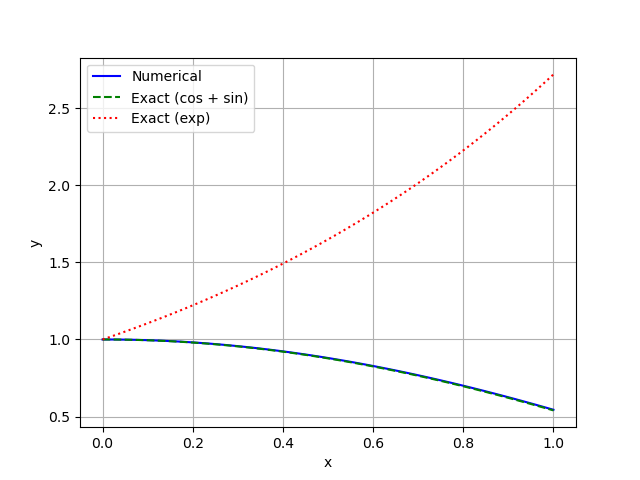
\includegraphics[scale=0.6]{fig.png}
			\centering
		\end{figure}
	\end{frame}

\end{document}